\documentclass[20pt]{extarticle}
\RequirePackage{url}
\RequirePackage[leqno]{amsmath}
\usepackage{graphicx}
\begin{document}

\noindent 1. The circular orbits of satellites 1 and 2 coincide. Satellite 2 has
twice the mass of satellite 1. Compare their accelerations.

\vspace{20mm}

\includegraphics{figs/compare-satellites}

A. 1's acceleration is half as much.

B. 1's acceleration is the same as 2's.

C. 1's acceleration is twice as much as 2's.

D. It depends on the periods of their orbits.

\pagebreak

%======================================================================


\noindent 2. At which point is the earth's gravitational field 1/4 as strong as at P?

\vspace{20mm}

\includegraphics{figs/one-fourth-g}

\pagebreak

%======================================================================

\noindent 3. The large planet has 9 times more mass than the small one.
At which location is the gravitational field zero?

\vspace{20mm}

\includegraphics{figs/earth-moon-cancel}

\pagebreak

%======================================================================


\noindent 4. A wedge has been cut out of the earth to let us see inside it.
Points 1, 2, 3, and 4 all lie along the same radial line. Point 1 is at the
earth's center, 3 at its surface, and 2 in the interior of the earth at the
midpoint between 1 and 3.

Rank the points by the strength of their gravitational fields, from weakest
to strongest.

\includegraphics{figs/inside-outside}

A. 4, 3, 2, 1

B. 4, 2, 3, 1

C. 1, 4, 2, 3

D. 1, 2, 4, 3


\pagebreak

%======================================================================

\noindent 5. The dolphin is initially moving underwater, staying just below the surface, but it then coasts to
a halt and spends some time thinking about dolphin stuff. Describe the energy transformation.

\includegraphics{figs/dolphin-energy}

A. PE to heat

B. KE to PE and heat

C. KE and PE to heat

D. KE to heat


\pagebreak

%======================================================================


\noindent 6. Some buses in Switzerland contain massive flywheels that store
kinetic energy when the bus goes downhill, then release it when it needs to
go up again. If the velocity of the spinning wheel could be doubled, its
mass could be cut by a factor of

A. $\sqrt{2}$.

B. 2.

C. 4.

D. It would still have to have the same mass.



\pagebreak

%======================================================================

\noindent 7. Joe is asleep in the library.
The flea gets bored and leaps off of his arm. The flea's mass is smaller than
Joe's by a factor of $10^8$. After the flea is in the air, compare Joe's speed to the flea's.

\includegraphics{figs/flea}

A. Joe isn't moving, but the flea is.

B. Joe recoils at a speed $10^{-8}$ that of the flea.

C. Joe recoils at a speed $10^{-16}$ that of the flea.

D. The whole planet earth recoils at an unmeasurably small speed.

\pagebreak

%======================================================================

\noindent 8. We adopt the frame
of reference in which Joe is initially at rest.
After the flea jumps, describe the kinetic
energy of the recoiling planet earth.

\includegraphics{figs/flea}

A. The earth's KE is zero.

B. The earth gains much more KE than the flea.

C. The earth's larger mass and smaller speed give it the same KE as the flea.

D. The earth gains much less KE than the flea.

E. Energy is conserved, so the earth loses an amount of KE the same as what the flea gains.

{\tiny [Based on a question by Eric Mazur.]}

\pagebreak

%======================================================================

\end{document}
